%% LyX 2.2.4 created this file.  For more info, see http://www.lyx.org/.
%% Do not edit unless you really know what you are doing.
\documentclass[conference]{IEEEtran}
\usepackage[latin9]{inputenc}
\usepackage{array}
\usepackage{multirow}
\usepackage{amsmath}
\usepackage{amssymb}

\makeatletter

%%%%%%%%%%%%%%%%%%%%%%%%%%%%%% LyX specific LaTeX commands.
%% Because html converters don't know tabularnewline
\providecommand{\tabularnewline}{\\}

%%%%%%%%%%%%%%%%%%%%%%%%%%%%%% User specified LaTeX commands.
\IEEEoverridecommandlockouts
\usepackage{tikz}
\usetikzlibrary{shapes.geometric, arrows}
\usepackage{cite}
\usepackage{amsfonts}\usepackage{algorithm}
\usepackage{algpseudocode}
\usepackage{graphicx}
\usepackage{textcomp}
\usepackage{xcolor}
\usepackage{pgfplots}
\usepackage{subfigure}


\pgfplotsset{compat=1.9}

\pgfplotsset{
    % #1: index in the group(0,1,2,...)
    % #2: number of plots of that group
    bar group size/.style 2 args={
        /pgf/bar shift={%
                % total width = n*w + (n-1)*skip
                % -> subtract half for centering
                -0.5*(#2*\pgfplotbarwidth + (#2-1)*\pgfkeysvalueof{/pgfplots/bar group skip})  + 
                % the '0.5*w' is for centering
                (.5+#1)*\pgfplotbarwidth + #1*\pgfkeysvalueof{/pgfplots/bar group skip}},%
    },
    bar group skip/.initial=2pt,
    plot 0/.style={blue,fill=blue!30!white,mark=none},%
    plot 1/.style={red,fill=red!30!white,mark=none},%
    plot 2/.style={brown!60!black,fill=brown!30!white,mark=none},%
    plot 3/.style={brown!60!black,fill=brown!30!white,mark=none},%
}

\def\BibTeX{{\rm B\kern-.05em{\sc i\kern-.025em b}\kern-.08em
    T\kern-.1667em\lower.7ex\hbox{E}\kern-.125emX}}


\newcommand{\fs@norules}{\def\@fs@cfont{\bfseries}\let\@fs@capt\floatc@ruled
    \def\@fs@pre{}%
    \def\@fs@post{}%
    \def\@fs@mid{\kern3pt}%
    \let\@fs@iftopcapt\iftrue}


\tikzstyle{startstop} = [ellipse,minimum width=2cm, minimum height=1cm, text centered, draw=black, fill=white]
\tikzstyle{io} = [trapezium, trapezium left angle=70, trapezium right angle=110, minimum width=2cm, minimum height=1cm, text centered, draw=black, fill=white]
\tikzstyle{process} = [rectangle, minimum width=1cm, minimum height=1cm, text centered, draw=black, fill=white]
\tikzstyle{decision} = [diamond, minimum width=2cm, minimum height=1cm, text centered, draw=black, fill=white]
\tikzstyle{arrow} = [thick,->,>=stealth]

\newcommand{\T}{\rule{0pt}{2.6ex}}       % Top strut
\newcommand{\B}{\rule[-1.2ex]{0pt}{0pt}} % Bottom strut

\makeatother

\begin{document}
%%%%%%%%%%%%%%%%%%%%%%%%%%%%%%%%%%%%%%%%%%%%%%%%%%%%%%%%%%%%%%%%%%%%%%%%%%%%%%%%%%%
%%%%%%%%%%%%%%%%%%%%%%%%%%%%%%%%%%%%%% TITLE %%%%%%%%%%%%%%%%%%%%%%%%%%%%%%%%%%%%%%
%%%%%%%%%%%%%%%%%%%%%%%%%%%%%%%%%%%%%%%%%%%%%%%%%%%%%%%%%%%%%%%%%%%%%%%%%%%%%%%%%%%

\title{Improved Global Routing By Using A Star Algorithm}

\author{\IEEEauthorblockN{Abdulrahman Khalid\IEEEauthorrefmark{1}, Hossam Ahmed\IEEEauthorrefmark{2},
Mahmoud Mohamed\IEEEauthorrefmark{3} and Muhanad Atef\IEEEauthorrefmark{4}} \IEEEauthorblockA{Computer Engineering Dept., Faculty of Engineering, Cairo University\\
 Cairo, Egypt\\
 \IEEEauthorrefmark{1}abdulrahman.elshafei98@gmail.com, \IEEEauthorrefmark{2}hossamahmed201515@gmail.com,
\IEEEauthorrefmark{3}mmmacmp@gmail.com, \IEEEauthorrefmark{4}muhanad.atef23@gmail.com}}

\maketitle
%%%%%%%%%%%%%%%%%%%%%%%%%%%%%%%%%%%%%%%%%%%%%%%%%%%%%%%%%%%%%%%%%%%%%%%%%%%%%%%%%%%
%%%%%%%%%%%%%%%%%%%%%%%%%%%%%%%%%%%% ABSTRACT %%%%%%%%%%%%%%%%%%%%%%%%%%%%%%%%%%%%%
%%%%%%%%%%%%%%%%%%%%%%%%%%%%%%%%%%%%%%%%%%%%%%%%%%%%%%%%%%%%%%%%%%%%%%%%%%%%%%%%%%%
\begin{abstract}
In this paper VLSI routing is improved by improving global routing,
this can be done by using A-Star with heuristic cost function that
has parameters which affect the time taken by the router on changing
instead of Dijkstra's algorithm in finding path, which will reduce
time taken in this process and achieve the minimum wirelength, many
comparisons are taken in this paper with different algorithms to find
the optimum algorithm to be used to achieve both minimum wirelength
and minimum time taken. From the comparisons of the paper we can find
that using any algorithm is a trade off as when time taken is decreased,
the wirelength is increased and vice versa, so there is no algorithm
which is better from the other algorithms in general but using A-Star
algorithm with the heuristic function in finding path is a good approach
to be used in global routing as it decreases the routing time and
achieve the minimum wirelength. 
\end{abstract}

%%%%%%%%%%%%%%%%%%%%%%%%%%%%%%%%%%%%%%%%%%%%%%%%%%%%%%%%%%%%%%%%%%%%%%%%%%%%%%%%%%%
%%%%%%%%%%%%%%%%%%%%%%%%%%%%%%%%%%%% KEY WORDS %%%%%%%%%%%%%%%%%%%%%%%%%%%%%%%%%%%%
%%%%%%%%%%%%%%%%%%%%%%%%%%%%%%%%%%%%%%%%%%%%%%%%%%%%%%%%%%%%%%%%%%%%%%%%%%%%%%%%%%%
\begin{IEEEkeywords}
VLSI Routing, Global Routing, Routing Algorithms, Fast Global Routing,
Fast Routing Algorithms, Routing Algoritms Comparisons. 
\end{IEEEkeywords}

%%%%%%%%%%%%%%%%%%%%%%%%%%%%%%%%%%%%%%%%%%%%%%%%%%%%%%%%%%%%%%%%%%%%%%%%%%%%%%%%%%%
%%%%%%%%%%%%%%%%%%%%%%%%%%%%%%%%%% INTRODUCTION %%%%%%%%%%%%%%%%%%%%%%%%%%%%%%%%%%%
%%%%%%%%%%%%%%%%%%%%%%%%%%%%%%%%%%%%%%%%%%%%%%%%%%%%%%%%%%%%%%%%%%%%%%%%%%%%%%%%%%%

\section{Introduction}

Routing is critical step in physical design process. Until now the
optimum solution for VLSI routing has not been achieved yet, so it
is considered as a very interesting challenging field. It is exactly
done in two steps, global routing and detailed routing. At first global
routing is run which is the responsible for making an approximate
routing for the whole circuit in order to be used as a guide for detailed
routing, then the detailed routing is run to make the exact routing
for the system. That means if global or detailed routing is improved
the whole routing process is improved, but there are many problems
that have to be overcame to make a correct routing process. First
of all the scale has to be taken into consideration, as millions of
wires exist in a small chip area which means that many kilometers
of wires are placed in a very small area, so wetotal wirelength has
to be minimized as much as possible, also it is known that as the
wirelength increases the resistance increases as well which means
more delay in the chip. There is another problem as circuits are made
in nano-scale which means that its geometric will be complex. Another
problem is that routing algorithm have to be applicable for more than
one layer with different costs. The direction of wires also have to
taken into consideration as the direction of wires in every layer
can be either vertical or horizontal and no diagonal paths, then to
go from source 'S' to target 'T' the path taken should be in (vertical
\textbar{} horizontal) directions that specified by the layer (at
each layer wires are placed in one direction only), then there is
another problem as when a wire goes from layer to another to continue
on the perpendicular direction it have to go through via which have
a high resistance. DFM (design for manufacturer) rules also has to
be achieved. All of these constraints must be taken into consideration
with the global routing to achieve hundred percent of the circuit
connections, that means global routing will take a lot of time to
achieve all these constraints, and here is the challenge to achieve
all the routing specifications with minimum time taken.

\begin{figure}
\centering \subfigure[Before routing]{ 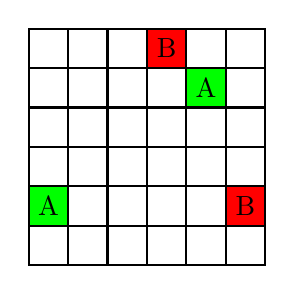
\begin{tikzpicture}[
            box/.style={rectangle,draw=black,thick, minimum size=0.5cm},
        ]
    
    \foreach \x in {0,0.5,...,2.5}{
        \foreach \y in {0,0.5,...,2.5}
            \node[box] at (\x,\y){};
    }
    \node [box,fill=green] at (0,0.5){A};
    \node[box,fill=green  ] at (2,2){A};  
    \node[box,fill=red  ] at (1.5,2.5){B}; 
    \node [box,fill=red] at (2.5,0.5){B}; 
    \end{tikzpicture} } \subfigure[Iteration number x]{ 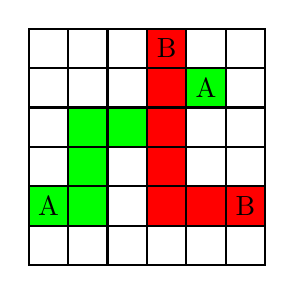
\begin{tikzpicture}[
            box/.style={rectangle,draw=black,thick, minimum size=0.5cm},
        ]
    
    \foreach \x in {0,0.5,...,2.5}{
        \foreach \y in {0,0.5,...,2.5}
            \node[box] at (\x,\y){};
    }
    
    \node [box,fill=green] at (0,0.5){A};
    \node[box,fill=green  ] at (2,2){A};  
    \node[box,fill=green  ] at (0.5,0.5){};  
    \node[box,fill=green  ] at (0.5,1){};  
    \node[box,fill=green  ] at (0.5,1.5){};  
    \node[box,fill=green  ] at (1,1.5){};  
    \node[box,fill=red  ] at (1.5,2.5){B}; 
    \node [box,fill=red] at (2.5,0.5){B};
    \node [box,fill=red] at (2,0.5){};
    \node [box,fill=red] at (1.5,0.5){};
    \node [box,fill=red] at (1.5,1){};
    \node [box,fill=red] at (1.5,1.5){};
    \node [box,fill=red] at (1.5,2){};
    \end{tikzpicture} } \subfigure[Iteration number y]{ 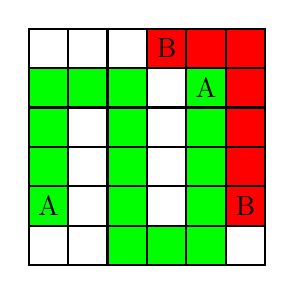
\begin{tikzpicture}[
            box/.style={rectangle,draw=black,thick, minimum size=0.5cm},
        ]
    
    \foreach \x in {0,0.5,...,2.5}{
        \foreach \y in {0,0.5,...,2.5}
            \node[box] at (\x,\y){};
    }
    
    \node [box,fill=green] at (0,0.5){A};
    \node[box,fill=green  ] at (2,2){A};  
    \node[box,fill=green  ] at (0,1){};  
    \node[box,fill=green  ] at (0,1.5){};  
    \node[box,fill=green  ] at (0,2){};  
    \node[box,fill=green  ] at (0.5,2){};  
    \node[box,fill=green  ] at (1,2){};  
    \node[box,fill=green  ] at (1,1.5){};  
    \node[box,fill=green  ] at (1,1){};  
    \node[box,fill=green  ] at (1,0.5){};  
    \node[box,fill=green  ] at (1.5,0){};  
    \node[box,fill=green  ] at (1,0){};  
    \node[box,fill=green  ] at (2,0){};  
    \node[box,fill=green  ] at (2,0.5){};  
    \node[box,fill=green  ] at (2,1){};  
    \node[box,fill=green  ] at (2,1.5){};  
    \node[box,fill=red  ] at (1.5,2.5){B}; 
    \node [box,fill=red] at (2.5,0.5){B};  
    \node [box,fill=red] at (2.5,1){};
    \node [box,fill=red] at (2.5,1.5){};
    \node [box,fill=red] at (2.5,2){};
    \node [box,fill=red] at (2.5,2.5){};
    \node [box,fill=red] at (2,2.5){};
    \end{tikzpicture} } \subfigure[After N iteration]{ 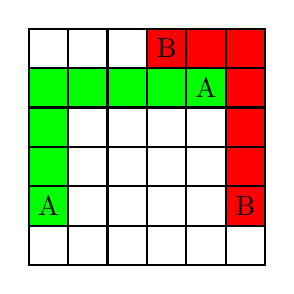
\begin{tikzpicture}[
            box/.style={rectangle,draw=black,thick, minimum size=0.5cm},
        ]
    
    \foreach \x in {0,0.5,...,2.5}{
        \foreach \y in {0,0.5,...,2.5}
            \node[box] at (\x,\y){};
    }
    
    \node [box,fill=green] at (0,0.5){A};
    \node[box,fill=green  ] at (2,2){A};  
    \node[box,fill=green  ] at (0,1){};  
    \node[box,fill=green  ] at (0,1.5){};  
    \node[box,fill=green  ] at (0,2){};  
    \node[box,fill=green  ] at (0.5,2){};  
    \node[box,fill=green  ] at (1,2){};  
    \node[box,fill=green  ] at (1.5,2){};  
    \node[box,fill=red  ] at (1.5,2.5){B}; 
    \node [box,fill=red] at (2.5,0.5){B}; 
    \node [box,fill=red] at (2.5,1){};
    \node [box,fill=red] at (2.5,1.5){};
    \node [box,fill=red] at (2.5,2){};
    \node [box,fill=red] at (2.5,2.5){};
    \node [box,fill=red] at (2,2.5){};
    \end{tikzpicture} } \caption{Finding path in global routing}
\label{fig:GlobalRoutingProcess} 
\end{figure}

Figure~\ref{fig:GlobalRoutingProcess} shows a very simple approach
of how the global router works. At (a) the source and target of both
(A,B) need to be connected ignoring obstacles, nevertheless we can
observe that the global router have to iterate to get the best routing
paths, at (b) (B,B) connected but there is no way to connect (A,A)
as when (B,B) connected together they blocked the way for (A,A) to
be connected, after some iterations we can find the figure at (c)
in which (A,A) and (B,B) connected correctly, but there is a problem,
the (A,A) connection is not the optimal path as there are paths which
achieve less wirelength, so the global router have to iterate until
reaching the optimal path. These iterations are done for only two
connections in one layer without obstacles, then how about millions
of wires in VLSI? this shows how much the global routing algorithm
has to be very fast in order to connect this huge number of wires
as fast as possible.

%%%%%%%%%%%%%%%%%%%%%%%%%%%%%%%%%%%%%%%%%%%%%%%%%%%%%%%%%%%%%%%%%%%%%%%%%%%%%%%%%%%
%%%%%%%%%%%%%%%%%%%%%%%%%%%%%%%%%% RELATED WORK %%%%%%%%%%%%%%%%%%%%%%%%%%%%%%%%%%%
%%%%%%%%%%%%%%%%%%%%%%%%%%%%%%%%%%%%%%%%%%%%%%%%%%%%%%%%%%%%%%%%%%%%%%%%%%%%%%%%%%%

\section{Related Work}

Several papers proposed various types of approaches to improve the
routing process, each of them tried to improve the overall routing
by improving one or more parameters, some paperes tried to decrease
number of vias, other papers tried to decrease the time taken and
so on. In \cite{b2} they used a sequential global routing and they
provided two bounded length maze algorithms as finding path algorithms
in order to make the router faster and to avoid congestions thus avoiding
overflow, the first one is optimal-BLMR and the second one is heuristic-BLMR.
optimal-BLMR is used to get the minimum cost paths to be used as a
routing paths, this can be done in three steps. First BLC (bounded
length constraint) is defined as a grater number than Manhattan distance
then to go from source to target the neighbour points are tested if
it can be a part of path or not, each point that violates the BLC
constraint is discarded. Second if the route started from point \textit{v}
and ended at point \textit{u} and there was many paths between these
two points, the normal maze algorithm wwill take the path with minimum
cost which may cause the route get into congestions, bun in optimal-BLMR
they keep track of all paths between these two points in order to
choose the path that will not cause overflow, it iterates on the minimum
cost path everytime and if it found a suitable path it reserves that
path otherwise it discard that path. Third step the optimal-BLMR iterates
on the reserved paths and choose the one to be used for routing. In
heuristic-BLMR they tried to speed the router up by reserving only
one path between the two points, but they also wanted to keep the
advantage of optimal-BLMR (avoidng congestions) and this can be achieved
by choosing the selected path only if the wirelength is enough to
detour around congested regions. The advantages of this paper are
using sequential global routing which is based on multithreaded global
routing which speedup the router, avoiding collision by using optimal-BLMR,
and making a fast and nearly avoiding collision algorithm (heuristic-BLMR).
But there are some disadvanatges too, as optimal-BLMR is very slow
to be used, although heuristic-BLMR is faster than optimal-BLMR its
results are not accurate as the wirelength is not the best compared
with other papers.

%%%%%%%%%%%%%%%%%%%%%%%%%%%%%%%%%%%%%%%%%%%%%%%%%%%%%%%%%%%%%%%%%%%%%%%%%%%%%%%%%%%
%%%%%%%%%%%%%%%%%%%%%%%%%%%%%% EXPERIMENTAL ANALYSIS %%%%%%%%%%%%%%%%%%%%%%%%%%%%%%
%%%%%%%%%%%%%%%%%%%%%%%%%%%%%%%%%%%%%%%%%%%%%%%%%%%%%%%%%%%%%%%%%%%%%%%%%%%%%%%%%%%

\section{Experimental Analysis}

we implement global routing with A\_Star router algorithm in c++ language
with Rsyn to parse input test cases files with format LEF/DEF. All
experiments are perfromed on a Machine with 2 GHZ intel Processor
and 8 GB RAM. our algorithm is focus on three important factors :total
wire-lenght, channel congestion ,number of vias. Our target is to
minimize a convex combination of the total wire-lenght and the number
of vias that represent the bends in the tree that result in solving
the net of pins to be connected.our test cases input are all from
ICCAD'19 contest for global routing.we test our code with different
heurestic function -that affect the run time of A{*}- to check its
effect on CPU time.our concern is on wire-lengh and number of vias
result from routing.

\subsubsection{Experiment1}

in this experiment we compare run time of router with dijkstra Router
and out A{*} router with heurestic function with differents constants
of heurestic functions that affect the run time of the router:

{\scriptsize{}$Heurestic-Fucntion1=(|p_{1}.x-p_{2}.x|+|p_{1}.y-p_{2}.y|*const1)+(|p_{1}.layer-p_{2}.layer|)*const2)$}{\scriptsize\par}

{\scriptsize{}$Heurestic-Fucntion2=(ln(|p_{1}.x-p_{2}.x|+|p_{1}.y-p_{2}.y|)*const1)+(|p_{1}.layer-p_{2}.layer|)*const2)$}{\scriptsize\par}

{\scriptsize{}$Heurestic-Fucntion3=(|p_{1}.x-p_{2}.x|+|p_{1}.y-p_{2}.y|*const1)+(ln(|p_{1}.layer-p_{2}.layer|)*const2)$}{\scriptsize\par}

{\tiny{}}
\begin{table}
{\tiny{}\caption{Compare run time of Dijkstra router and A{*} router with different
heuristic function}
}{\tiny\par}

{\tiny{}}%
\begin{tabular}{|c|c|c|c|c||c|c|c|c|}
\hline 
\multirow{3}{*}{{\tiny{}Design}} & \multicolumn{8}{c|}{{\tiny{}A{*} Router}}\tabularnewline
\cline{2-9} 
 & \multicolumn{4}{c||}{{\tiny{}F1}} & \multicolumn{4}{c|}{{\tiny{}F2}}\tabularnewline
\cline{2-9} 
 & {\tiny{}(0.1,0.1)} & {\tiny{}(0.2,0.1)} & {\tiny{}(0.3,0.3)} & {\tiny{}(0.5,0.5)} & {\tiny{}(0.1,0.1)} & {\tiny{}(0.2,0.1)} & {\tiny{}(0.3,0.3)} & {\tiny{}(0.5,0.5)}\tabularnewline
\hline 
\hline 
{\tiny{}19test2} & {\tiny{}87.150469} & {\tiny{}75.843764} & {\tiny{}87.797614} & {\tiny{}87.086193} & {\tiny{}90.440165} & {\tiny{}93.288501} & {\tiny{}89.414646} & {\tiny{}96.377979}\tabularnewline
\hline 
{\tiny{}19test3} & {\tiny{}2.489458} & {\tiny{}2.511599} & {\tiny{}2.606054} & {\tiny{}2.874605} & {\tiny{}2.461400} & {\tiny{}2.469304} & {\tiny{}2.480592} & {\tiny{}2.497377}\tabularnewline
\hline 
{\tiny{}19test5} & {\tiny{}13.785204} & {\tiny{}12.381436} & {\tiny{}14.959666} & {\tiny{}14.859677} & {\tiny{}12.264829} & {\tiny{}13.449206} & {\tiny{}12.039944} & {\tiny{}14.766495}\tabularnewline
\hline 
{\tiny{}sample} & {\tiny{}0.221261} & {\tiny{}0.075472} & {\tiny{}0.073069} & {\tiny{}0.073769} & {\tiny{}0.071577} & {\tiny{}0.157244} & {\tiny{}0.078624} & {\tiny{}0.072691}\tabularnewline
\hline 
{\tiny{}sample2} & {\tiny{}0.096618} & {\tiny{}0.073988} & {\tiny{}0.072911} & {\tiny{}0.074165} & {\tiny{}0.078316} & {\tiny{}0.090906} & {\tiny{}0.071333} & {\tiny{}0.072767}\tabularnewline
\hline 
{\tiny{}sample3} & {\tiny{}7.002814} & {\tiny{}6.948016} & {\tiny{}6.266789} & {\tiny{}5.198969} & {\tiny{}6.893310} & {\tiny{}6.400888} & {\tiny{}6.974920} & {\tiny{}6.906992}\tabularnewline
\hline 
\end{tabular}{\tiny\par}
\end{table}
{\tiny\par}

\begin{table}

{\tiny{}\caption{Continue compare run time of Dijkstra router and A{*} router with
different heuristic function}
}{\tiny\par}

{\tiny{}}%
\begin{tabular}{|c|c|c|c|c|c|}
\hline 
\multirow{3}{*}{{\tiny{}Design}} & \multicolumn{4}{c|}{{\tiny{}A{*} Router}} & \multirow{3}{*}{{\tiny{}Dijkstra}}\tabularnewline
\cline{2-5} 
 & \multicolumn{4}{c|}{{\tiny{}F3}} & \tabularnewline
\cline{2-5} 
 & {\tiny{}(0.1,0.1)} & {\tiny{}(0.2,0.1)} & {\tiny{}(0.3,0.3)} & {\tiny{}(0.5,0.5)} & \tabularnewline
\hline 
\hline 
{\tiny{}19test2} & {\tiny{}86.598509} & {\tiny{}83.204272} & {\tiny{}103.166426} & {\tiny{}102.378304} & {\tiny{}91.348007}\tabularnewline
\hline 
{\tiny{}19test3} & {\tiny{}2.481847} & {\tiny{}2.486656} & {\tiny{}3.622759} & {\tiny{}2.556863} & {\tiny{}3.435606}\tabularnewline
\hline 
{\tiny{}19test5} & {\tiny{}12.655603} & {\tiny{}15.447421} & {\tiny{}15.629251} & {\tiny{}20.004493} & {\tiny{}11.824573}\tabularnewline
\hline 
{\tiny{}sample} & {\tiny{}0.073731} & {\tiny{}0.070911} & {\tiny{}0.073468} & {\tiny{}0.103421} & {\tiny{}0.071829}\tabularnewline
\hline 
{\tiny{}sample2} & {\tiny{}0.078171} & {\tiny{}0.079362} & {\tiny{}0.088107} & {\tiny{}0.099699} & {\tiny{}0.071945}\tabularnewline
\hline 
{\tiny{}sample3} & {\tiny{}6.470339} & {\tiny{}7.195767} & {\tiny{}8.455288} & {\tiny{}7.637577} & {\tiny{}7.038505}\tabularnewline
\hline 
\end{tabular}{\tiny\par}

\end{table}

we notice from Table 1,Table 2 that heurestric function affect run
time of router ,decreases it to be lower than dijkstra router's run
time in many test cases. run time changes with the change of heuristic
function constants. we notice that higher constants increase the run
time and sometimes be greater than dijkstra router's runtime. Heurestic
function 2 has ovarall results which is good than others herestics
function, with other Heurestic functions run time may improve mostly. 

\subsection{Performance Comparsions}

we compare results of our algorithm which focus on factors - total
wire-lenght,number of vias in the routing results - with TripleZ and
NTUidRoute algorithms in ICCAD'19 Table 3 .threads number used in
all cases is 8 threads. score used as unit to compare ,score of wire
length is a function of metal pitch and wire length and weight:

$WLScore=\frac{wire-length*weight}{metal-pitch}$

score of vias is function of number of vias :

$ViasScore=\#vias*2$

{\tiny{}}
\begin{table}
{\tiny{}\caption{compared Wire Lengh,vias with TripleZ and NTUidRoute Algorithms in
ICCAD'19 Global routing Contest }
}{\tiny\par}

{\tiny{}}%
\begin{tabular}{|c|c|c|c|c|c|c|}
\hline 
\multirow{2}{*}{{\tiny{}Design}} & \multicolumn{3}{c|}{{\tiny{}wire-length scores}} & \multicolumn{3}{c|}{{\tiny{}vias score}}\tabularnewline
\cline{2-7} 
 & {\tiny{}TripleZ} & {\tiny{}NTUidRoute} & {\tiny{}ours} & {\tiny{}TripleZ} & {\tiny{}NTUidRoute} & {\tiny{}ours}\tabularnewline
\hline 
{\tiny{}19test2} & {\tiny{}12485549.76} & {\tiny{}12992510.61} & {\tiny{}12150100} & {\tiny{}3261476.00} & {\tiny{}4017448.00} & {\tiny{}2803560}\tabularnewline
\hline 
{\tiny{}19test3} & {\tiny{}569622.01} & {\tiny{}466809.64} & {\tiny{}389460} & {\tiny{}251728.00} & {\tiny{}318404.00} & {\tiny{}176728}\tabularnewline
\hline 
{\tiny{}19test4} & {\tiny{}17800019.36} & {\tiny{}15935101.91} & {\tiny{}14663400} & {\tiny{}4265744.00} & {\tiny{}4789488.00} & {\tiny{}2666120}\tabularnewline
\hline 
{\tiny{}19test5} & {\tiny{}2859212.04} & {\tiny{}2495661.79} & {\tiny{}2851900} & {\tiny{}695348.00} & {\tiny{}771328.00} & {\tiny{}446024}\tabularnewline
\hline 
{\tiny{}19test7} & {\tiny{}74264784.88} & {\tiny{}65028116.52} & {\tiny{}70041500} & {\tiny{}19689760.00} & {\tiny{}23183264.00} & {\tiny{}12532800}\tabularnewline
\hline 
{\tiny{}Avg} & {\tiny{}21595837.61} & {\tiny{}19383640} & {\tiny{}20019272} & {\tiny{}5632811.2} & {\tiny{}6615986.4} & {\tiny{}3725046.4}\tabularnewline
\hline 
\end{tabular}{\tiny\par}
\end{table}
{\tiny\par}

\subsection{Observation}

our algorithm has wire-length score less than TripleZ with 7.3\% and
greater than NTUidRoute with 3.28\% but it affect the vias number
greatly that our vias score is less than NTUidRoute's vias score by
43\%

%%%%%%%%%%%%%%%%%%%%%%%%%%%%%%%%%%%%%%%%%%%%%%%%%%%%%%%%%%%%%%%%%%%%%%%%%%%%%%%%%%%
%%%%%%%%%%%%%%%%%%%%%%%%%%%%%%%%%%% Conclusion and Future Work %%%%%%%%%%%%%%%%%%%%%%%%%%%%%%%%%%%
%%%%%%%%%%%%%%%%%%%%%%%%%%%%%%%%%%%%%%%%%%%%%%%%%%%%%%%%%%%%%%%%%%%%%%%%%%%%%%%%%%%

\section{Conclusion and Future Work}

The goal of this paper is to develop A-star-based global Router with
minimum wirelength and number of vias as the more vias number the
more heat generated from the chip with minimum run time.to overcome
the time problem we use heurestic function that decrease the run time
of router and test it with different constants to define its affect
on run time ,for future work we aim to define effective heurestic
function to improve run time and using more effecient versions of
A\_star algorithm such as bi-directional A-star ,deep A-star,iterative
deeping A-star .for instance bi-directional A-star that process edges
in both directions that improve run time.

%%%%%%%%%%%%%%%%%%%%%%%%%%%%%%%%%%%%%%%%%%%%%%%%%%%%%%%%%%%%%%%%%%%%%%%%%%%%%%%%%%%
%%%%%%%%%%%%%%%%%%%%%%%%%%%%%%%%%%%% REFERENCES %%%%%%%%%%%%%%%%%%%%%%%%%%%%%%%%%%%
%%%%%%%%%%%%%%%%%%%%%%%%%%%%%%%%%%%%%%%%%%%%%%%%%%%%%%%%%%%%%%%%%%%%%%%%%%%%%%%%%%%
\begin{thebibliography}{1}
\bibitem{b1} Muhammet Mustafa Ozdal and M. D. F. Wong, \char`\"{}Archer:
a history-driven global routing algorithm,\char`\"{} \textit{2007
IEEE/ACM International Conference on Computer-Aided Design}, San Jose,
CA, 2007, pp. 488-495, doi: 10.1109/ICCAD.2007.4397312.

\bibitem{b2} Liu, Wen-Hao, et al. \char`\"{}NCTU-GR 2.0: Multithreaded
collision-aware global routing with bounded-length maze routing.\char`\"{}
\textit{IEEE Transactions on computer-aided design of integrated circuits
and systems} 32.5 (2013): 709-722.
\end{thebibliography}

\end{document}
